\chapter{内存管理}



\paragraph{}
\paragraph{}
\paragraph{}
\paragraph{}
\paragraph{}
\paragraph{}
\paragraph{}
\paragraph{}
\paragraph{}
\paragraph{}











\section{没有高速缓存的转换过程}

在没有高速缓存的情况下虚拟地址的转换过程:

\begin{figure}[htbp]
\begin{center}
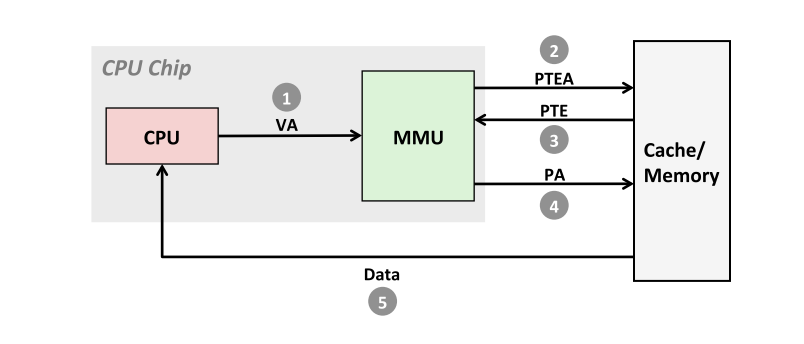
\includegraphics[width=1\textwidth]{slowvava.png}
\caption{没有高速缓存对数据的访问}
\end{center}
\end{figure}

\begin{enumerate}
\item Processor sends virtual address to MMU
\item MMU fetches PTE from page table in memory(Access memory once)
\item MMU sends physical address to memory(Access memory twice)
\item Memory send sdata word to processor	
\end{enumerate}

因此在没有高速缓存的情况下,CPU读取数据会进行2次内存访问,其中1次读取页表,1次读取数据。

\section{有高速缓存的转换过程}

在有高速缓存的情况下虚拟地址的转换过程:


\begin{enumerate}
\item 处理器将虚拟地址发送给MMU
\item MMU根据PTEA从cache中读取pte,如果命中cache则使用转换出的物理地址读取内存数据。
\item 如果没有命中cache,则重内存中取得pte并更新cache,再重内存中读取数据(最多读取2次内存)
\end{enumerate}


\begin{figure}[!htbp]
\begin{center}
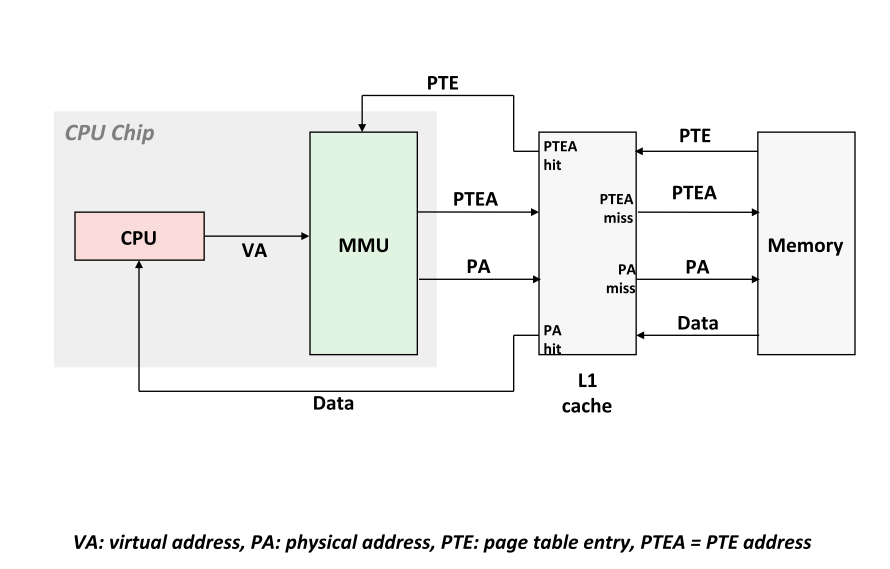
\includegraphics[width=1\textwidth]{highvava.png}
\caption{有高速缓存时对数据的访问}
\end{center}
\end{figure}

由于局部性原理,cache命中的概率很高,这样就减少了对内存的直接访问,从而提高了访问速度。



\section{not named}
\begin{figure}[htbp]
\begin{center}
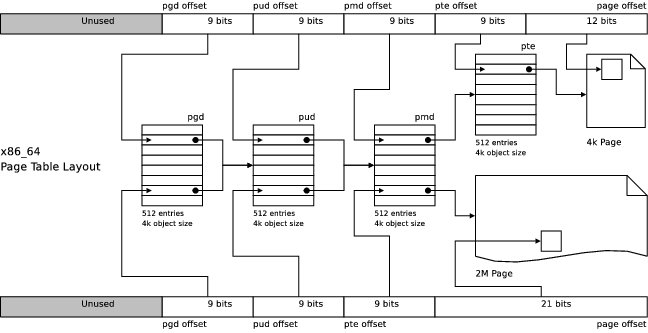
\includegraphics[width=1\textwidth]{va-to-pa.png}
\caption{虚拟地址转换\cite{linuxmm}}
\end{center}
\end{figure}


\section{PTE结构}
\begin{figure}[htbp]
\begin{center}
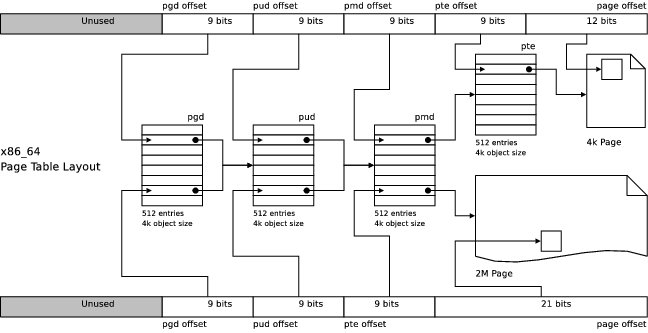
\includegraphics[width=1\textwidth]{va-to-pa.png}
\caption{PTE结构\cite{linuxmm}}
\end{center}
\end{figure}



Core i7的页表结构:

\begin{figure}[htbp]
\begin{center}
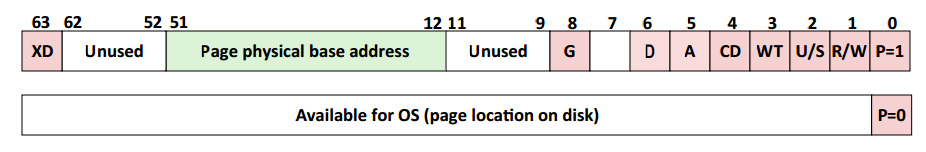
\includegraphics[width=1\textwidth]{pte.png}
\caption{Core i7 Level 4 Page Table	Entries}
\end{center}
\end{figure}


\begin{itemize}
\item \textbf{P:} Child page is present in memory (1)or not(0)	
\item \textbf{R/W:} Read-only or read-write access permission for child page	
\item \textbf{U/S:} User or	supervisor mode	access	
\item \textbf{WT:} Write-through or	write-back cache policy for this page	
\item \textbf{CD:} Cache disabled (1) or	enabled (0)	
\item \textbf{A:} Reference bit (set by MMU on reads and	writes, cleared	by sohware)		
\item \textbf{D:} Dirty bit (set	by MMU on writes, cleared by sohware)	
\item \textbf{G:} Global	page (don’t	evict from TLB on task switch)	
\item \textbf{Page physical base address:} 40 most significant bits of physical page address (forces pages to be	4KB	aligned)	
\end{itemize}




\section{写时复制(COW)}
